% ----------------------------------------------------------------
% Article Class (This is a LaTeX2e document)  ********************
% ----------------------------------------------------------------
\documentclass[11pt]{article}
\usepackage[english]{babel}
\usepackage{amsmath,amsthm, amssymb}
\usepackage{amsfonts}
\usepackage{multirow}
\usepackage{threeparttable}

%Candelaria's favorite packages
\usepackage{setspace}	% Set the spacing for the document
\usepackage{xtab}		% Use for tables
\usepackage{comment}	% Use for block comments
\usepackage{rotating}	% Helpful for rotating figures
\usepackage{lscape}	% Change a page into landscape
\usepackage{hyperref}
\hypersetup{colorlinks=false,pdfborder={0 0 0},breaklinks=true}
\usepackage{graphicx}	% Load a graphic image
%\usepackage{url}		% Use for formatting URLS (nice for NatBib also)
\usepackage{booktabs}  	% Use for nice tables/ Works well with ESTOUT
\usepackage{longtable} 	% Used to break long tables over multiple pages
\usepackage{caption}
\usepackage{subcaption} 	% Used to create SubFloats
\usepackage{listings} 	% Use to enter code blocks, like a fancy verbatim

% ADD COLOR:
\usepackage{color}
\usepackage[usenames, dvipsnames, svgnames, table]{xcolor}

% Packages for the bibliography
\usepackage[longnamesfirst]{natbib}
%\usepackage{natbib}

% Set Page Margins
%\usepackage{fullpage}
\addtolength{\oddsidemargin}{-.875in}
\addtolength{\evensidemargin}{-.875in}
\addtolength{\textwidth}{1.75in}
\addtolength{\topmargin}{-.875in}
\addtolength{\textheight}{1.75in}

% Set line and table spacing
\renewcommand{\baselinestretch}{1.0}
\renewcommand{\arraystretch}{1.1}
\setlength\abovedisplayskip{0pt}
\setlength\belowdisplayskip{0pt}

% Redefine the cite command
\renewcommand\cite{\citet}

%\setlength{\parindent}{0in}

%\setlength{\leftmargin}{0pt} \setlength{\parskip}{1.1ex} \setlength{\parindent}{1em} \setlength{\itemsep}{0pt} \setlength{\footnotesep}{10pt}
%\renewcommand{\footnoterule}{\rule{3in}{.3pt}\vspace{-.3pt}}

% THEOREMS -------------------------------------------------------
\newtheorem{thm}{Theorem}[section]
\newtheorem{cor}[thm]{Corollary}
\newtheorem{lem}[thm]{Lemma}
\newtheorem{prop}[thm]{Proposition}
\theoremstyle{definition}
\newtheorem{defn}[thm]{Definition}
\theoremstyle{remark}
\newtheorem{rem}[thm]{Remark}
%\numberwithin{equation}{section} %Number equations within section
% ----------------------------------------------------------------

%%%%%%TYPESET LINEAR EQUATIONS
\usepackage{environ}

\makeatletter

\newcommand{\LinearSystems@SetupLets}{%
  \let\col=&%
  \let\+=+%
  \let\-=-%
  \let\===%
}
\newcommand{\LinearSystems@SetupCatcodes}{%
  \catcode`\&=\active
  \catcode`\+=\active
  \catcode`\-=\active
  \catcode`\==\active
}
\newcommand{\LinearSystems@Setup}{}
\begingroup
  \LinearSystems@SetupCatcodes
  \gdef\LinearSystems@Setup{%
    \LinearSystems@SetupLets
    \LinearSystems@SetupCatcodes
    \newcommand&[1][0pt]{\col\hspace{##1}\col}%
    \def+{\col\+{}{}\col}%
    \def-{\col\-{}{}\col}%
    \def={\col\={}{}\col}%
  }
\endgroup

\NewEnviron{LinearSystems}[1]{\begin{alignat*}{#1}\BODY\end{alignat*}}
\let\LinearSystems@OriginalBegin\LinearSystems
\def\LinearSystems{\LinearSystems@Setup\LinearSystems@OriginalBegin}

\makeatother


%%%%%%%%%%%%%%%%%%%%%%%%%%%
%% COMMANDS FOR JUSTIFYING MATRIX ELEMENTS AND FOR CREATING
%% AUGMENTED MATRICES
% The following code redefines the matrix environment, such
% that we can left or right justify the contents in a matrix 

\makeatletter
\renewcommand*\env@matrix[1][*\c@MaxMatrixCols c]{%
  \hskip -\arraycolsep
  \let\@ifnextchar\new@ifnextchar
  \array{#1}}
\makeatother
%%%%%%%%%%%%%%%%%%%%%%%%

\begin{document}

\begin{center}
{\huge Linear Algebra Lecture Notes\footnote{This lecture is a slightly modified version of one written by Luigi Pistaferri. If you find errors, please let us know so that we may correct them. Thanks!}} \\[5pt]
{\Large Stanford GSE Math Camp 2019 \\[5pt]
Do Not Distribute Outside GSE}
\end{center}

\section{Matrices}
\begin{itemize}
\item A \textbf{matrix} is a rectangular set of elements ordered in rows and columns:
$$
\textbf{A} =
\begin{pmatrix}
a_{11}&a_{12}&...&a_{1C}\\
a_{21}&a_{22}&...&a_{2C}\\
...&...&...&...\\
a_{R1}&a_{R2}&...&a_{RC}\\
\end{pmatrix}
$$
In this matrix there are R rows and C columns.
\item If R = C this matrix is a \textbf{square} matrix, otherwise it is \textbf{rectangular}.
\begin{itemize}
\item The upper left to lower right \textbf{diagonal} of a square matrix is called the \textbf{main} or \textbf{principal} diagonal if it is square. Sometimes this is indicated as $diag(\mathbf{A})$
\item The lower left to upper right diagonal of a square matrix is called the \textbf{opposite} diagonal.
\end{itemize}
\item The generic element of the matrix is $a_{ij}$. The first subscript $i$ indexes the row where this element is located. The second subscript indexes the column $j$ where this element is located. So $a_{25}$ is the element in the 2nd row and the 5th column of the matrix \textbf{A}.
\item A matrix is said to be \textbf{symmetric} if $a_{ij}=a_{ji}$.
\item The dimension of a matrix is defined by the number of rows and columns it has. So, a matrix with R rows and C columns has dimension $(R \times C)$. This will sometimes be written under the \textbf{A}, but is often omitted. The dimension of a matrix \textbf{A} is indicated as $dim(\mathbf{A})$.
\item A \textbf{vector} is a particular type of matrix with either one row (in which case it is called a row vector) or one column (called a column vector). A vector is conventionally assumed to be a column vector if it is not otherwise indicated.

$$
\textbf{B} =
\begin{pmatrix}
b_{11}&b_{12}&...&b_{1C}\
\end{pmatrix}
$$

$$
\textbf{D} =
\begin{pmatrix}
d_{11}\\
d_{21}\\
...\\
d_{R1}\\
\end{pmatrix}
$$

Above, \textbf{B} is a row vector and \textbf{D} is a column vector.
\item A \textbf{scalar} is a particular type of matrix with just one row and one column, i.e. a singleton.
\end{itemize}

%%%%%%%%%%%%%%%%%%%%%%%%%%%%
%%%%%%%%%%%%%%%%%%%%%%%%%%%%
\section{Solving Linear Systems of Equations with Matrices}
%%%%%%%%%%%%%%%%%%%%%%%%%%%%
%%%%%%%%%%%%%%%%%%%%%%%%%%%%
\begin{itemize}
\item \textbf{Quick Review of Elementary Equation Operations} The following operations are used to transform the equations of a linear system, while maintaining an \textit{equivalent} linear system:
\begin{enumerate}
\item Interchange two equations
\item Multiply two sides of an equation by a constant
\item Add equations to each other
\end{enumerate}
By \textit{equivalence}, we me that the the same values of $x_j$ solve both the original and the transformed systems. 
\item \textbf{Quick Review of Gaussian Elimination}: Gaussian elimination is a method by which we start with some linear system of $m$ equations in $n$ unknowns and use the elementary equation operations to eliminate variables, until we arrive at an equivalent system of the form:
$$
\begin{matrix}[ccccccccccc]
\fbox{$a'_{11}x_1$} & + & a'_{12}x_2 & + & a'_{13}x_3 & + & \cdots & + & a'_{1n}x_n & = & b_1' \\
&  & \fbox{$a'_{22}x_2$} & + & a'_{23}x_3 & + & \cdots & + & a'_{2n}x_n & = & b'_2 \\
&  &  &  & \fbox{$a'_{33}x_3$} & + & \cdots & + & a'_{3n}x_n & = & b'_3 \\
&  &  &  &  &  & \vdots &  &  & \vdots &  \\
&  &  &  &  &  &  &  & \fbox{$a'_{mn}x_n$} & = & b'_m \\
\end{matrix}
$$
where $a'_{ij}$ denotes the coefficient of the $j$th unknown in the $i$th equation after performing elementary equation operations. At each stage of the elimination process, we want to change some coefficient of our system to 0 by adding a multiple of an earlier equation to the given equation. The coefficients \fbox{$a'_{11}$}, \fbox{$a'_{22}$}, etc. in the boxes are referred to as \textbf{pivots}\footnote{Pivots do not need to be on the $ij$ diagonal, where $i=j$. Also, there are times when we will eliminate variables in the rows above a pivot}, since they are the terms used to eliminate the variables in the rows below them in their respective columns. Once the linear system is in the above reduced form, we then use back substitution to find the values of the $x_j$s.      
\item \textbf{Quick review of Gauss-Jordan Elimination}: Gauss-Jordan Elimination  takes over where Gaussian Elimination left off. Once the linear system is in the \textit{reduced form}, as shown in the Gaussian Elimination section above, we use elementary equation operations and Gaussian elimination to
\begin{enumerate}
\item Change the coefficient of the pivot term in each equation to 1
\item Eliminate all terms above each pivot in its column
This process results in a reduced, equivalent system. For example, a system of $m$ equations in $m$ unknowns would look something like this:
$$
\begin{matrix}[ccccccccccc]
\fbox{$x_1$} &  &  &  &  &  &  &  &  & = & b_1^{*} \\
&  & \fbox{$x_2$} &  &  &  &  &  &  & = & b_2^{*} \\
&  &  &  & \fbox{$x_3$} &  &  &  &  & = & b_3^{*} \\
&  &  &  &  &  & \ddots &  &  & \vdots &  \\
&  &  &  &  &  &  &  & \fbox{$x_n$} & = & b_m^{*} \\
\end{matrix}
$$
\end{enumerate}
Notice that we have fully solved for the $x_j$s.

\item \textbf{Back to Matrices...} Matrices provide an efficient way to represent linear systems such as 
\begin{equation*}
\begin{split}
a_{11} x_1 + a_{12} x_2 + \cdots + a_{1n} x_n &= b_1 \\
a_{21} x_1 + a_{22} x_2 + \cdots + a_{2n} x_n &= b_2 \\
\vdots \quad  \quad \quad \quad \vdots \quad \quad \quad \quad \vdots \\
a_{m1} x_1 + a_{m2} x_2 + \cdots + a_{mn} x_n &= b_m  \label{eq:genlinsys}
\end{split}
\end{equation*}
The above system of equations can be written compactly as:
$$
\mathbf{Ax = b}
$$
where
\begin{enumerate}
\item The $m \times n$ \textbf{coefficient matrix A} is an array of $mn$ real numbers arrange in $m$ rows by $n$ columns:
$$
\begin{pmatrix}
a_{11}&a_{12}&\cdots&a_{1n} \\
a_{21}&a_{22}&\cdots&a_{2n} \\
\vdots&\vdots&\ddots&\vdots \\
a_{n1}&a_{n2}&\cdots&a_{nn} \\
\end{pmatrix}
$$
\item The unknown quantities are represented by the vector 
$$
\mathbf{x} =
\begin{pmatrix}
x_1 \\
x_2 \\
\vdots \\
x_n
\end{pmatrix}$$
\item The right hand side of the linear system is represented by the vector 
$$
\mathbf{b} =
\begin{pmatrix}
b_1 \\
b_2 \\
\vdots \\
b_m
\end{pmatrix}
$$
\end{enumerate}
Putting this all together, we have:
$$
\begin{pmatrix}
a_{11}&a_{12}&\cdots&a_{1n} \\
a_{21}&a_{22}&\cdots&a_{2n} \\
\vdots&\vdots&\ddots&\vdots \\
a_{n1}&a_{n2}&\cdots&a_{nn} \\
\end{pmatrix}
\begin{pmatrix}
x_1 \\
x_2 \\
\vdots \\
x_n
\end{pmatrix}
 =
\begin{pmatrix}
b_1 \\
b_2 \\
\vdots \\
b_m
\end{pmatrix}
$$
\item We can solve a system of linear equations using an \textbf{Augmented Matrix}. When we append \textbf{b} to the coefficient matrix \textbf{A}, we get the augmented matrix $\widehat{\mathbf{A}} = [\mathbf{A}|\mathbf{b}]$
$$
\widehat{\mathbf{A}} =
\begin{pmatrix}[cccc|c]
a_{11}&a_{12}&\cdots&a_{1n} & b_1 \\
a_{21}&a_{22}&\cdots&a_{2n} & b_2 \\
\vdots&\vdots&\ddots&\vdots & \vdots \\
a_{n1}&a_{n2}&\cdots&a_{nn} & b_m \\
\end{pmatrix}
$$
Notice that the \textbf{x} vector is not explicitly represented in the augmented matrix. 
\item We can conduct \textbf{elementary row operations} to transform some augmented matrix representation of a linear system into another augmented matrix that represents an \textit{equivalent} linear system. Specifically, we can do the following:
\begin{enumerate}
\item Interchange two rows 
\item Multiply a row by a constant
\item Add two rows to each other
\end{enumerate}
Notice how similar these operations are when compared with elementary equation operations. Let's illustrate each of the row operations below.
\begin{itemize}
\item \textbf{Interchanging Rows}: Suppose we have the augmented matrix
$$
\widehat{\mathbf{A}} =
\begin{pmatrix}[cc|c]
a_{11}&a_{12} & b_1 \\
a_{21}&a_{22} & b_2 \\
\end{pmatrix}
$$
If we interchange the two rows, we get the following augmented matrix: 
$$
\begin{pmatrix}[cc|c]
a_{21}&a_{22} & b_2 \\
a_{11}&a_{12} & b_1 \\
\end{pmatrix}
$$
which represents a linear system \textit{equivalent} to the matrix $\widehat{\mathbf{A}}$.
\item \textbf{Multiplying by a Constant}: If we multiply the second row of matrix $\widehat{\mathbf{A}}$ by a constant $c$, we obtain the following augmented matrix
$$
\begin{pmatrix}[cc|c]
a_{11}&a_{12} & b_1 \\
ca_{21}&ca_{22} & cb_2 \\
\end{pmatrix}
$$
which represents a linear system \textit{equivalent} to the matrix $\widehat{\mathbf{A}}$.
\item \textbf{Adding Rows}: If we add the first row of matrix $\widehat{\mathbf{A}}$ to the second row, we obtain the following augmented matrix:
$$
\begin{pmatrix}[cc|c]
a_{11}&a_{12} & b_1 \\
a_{11}+a_{21}&a_{12}+a_{22} & b_1 + b_2 \\
\end{pmatrix}
$$
which represents a linear system \textit{equivalent} to the matrix $\widehat{\mathbf{A}}$.
\end{itemize}
\item \textbf{Row Echelon Form}: We use row operations to change coefficients in the augmented matrix to 0 and to put it in a matrix form representing the final linear system of Gaussian elimination. An augmented matrix of the form
$$
\begin{pmatrix}[ccccc|c]
\fbox{$a'_{11}$}&a'_{12} & a'_{13} &\cdots & a'_{1n} & b'_1 \\
0 & \fbox{$a'_{22}$} & a'_{23} & \cdots & a'_{2n} & b'_2 \\
0 & 0 & \fbox{$a'_{33}$} & \cdots & a'_{3n} & b'_3 \\
0 & 0 & 0 & \ddots & \vdots & \vdots \\
0 & 0 & 0 & 0 & \fbox{$a'_{mn}$} & b'_m \\
\end{pmatrix}
$$
is said to be in \textit{row echelon form}. Each row has more leading zeros than the row preceding it.
\item \textbf{Reduced Row Echelon Form}: Reduced row echelon form is the matrix representation of a linear system after Gauss-Jordan elimination. For a system of $m$ equations in $n$ unknowns, with no all-zero rows, the reduced row echelon form would be: 
$$
\begin{pmatrix}[ccccc|c]
\fbox{$1$}&0 & 0 &\cdots & 0 & b^{*}_1 \\
0 & \fbox{$1$} & 0 & \cdots & 0 & b^{*}_2 \\
0 & 0 & \fbox{$1$} & \cdots & 0 & b^{*}_3 \\
0 & 0 & 0 & \ddots & \vdots & \vdots \\
0 & 0 & 0 & 0 & \fbox{$1$} & b^{*}_m \\
\end{pmatrix}
$$
\end{itemize}

\section{Properties of Matrices}
\begin{enumerate}
\item Suppose you have two matrices \textbf{A} and \textbf{B} with generic elements $a_{ij}$ and $b_{ij}$. Then $\mathbf{A}=\mathbf{B}$ if and only if (also denoted iff) $a_{ij}=b_{ij}$ for all (also denoted $\forall$) $i, j$.
\item Suppose you have two matrices \textbf{A} and \textbf{B} with generic elements $a_{ij}$ and $b_{ij}$. You can add or subtract ($\textbf{A} \pm \textbf{B}$) them iff they have the same dimension. The resulting matric \textbf{C} has a generic element: $c_{ij} = a_{ij} \pm b_{ij}$.
\begin{itemize}
\item Example: Let \textbf{A} and \textbf{B} be defined:

$$
\textbf{A} =
\begin{pmatrix}
1&5\\
-2&3
\end{pmatrix}
$$

$$
\textbf{B} =
\begin{pmatrix}
-7&0\\
4&1\\
\end{pmatrix}
$$
Then 
$$
\textbf{A} + \textbf{B} =
\begin{pmatrix}
-6&5\\
2&4\\
\end{pmatrix}
$$
And
$$
\textbf{A} - \textbf{B} =
\begin{pmatrix}
8&5\\
-6&2\\
\end{pmatrix}
$$
\end{itemize}
\item Multiplying \textbf{A} by a scalar, $\lambda$ is always a feasible operation. The resulting matrix $\mathbf{B} = \lambda\mathbf{A}$ will have generic elements $b_{ij} = \lambda a_{ij}$.
\item A matrix can be \textbf{transposed}. This means exchanging the rows with the columns, i.e., creating a new matrix whose rows are the columns of the original matrix (and vice versa). If this original matrix is $\mathbf{A}$ its transpose is denoted $\mathbf{A'}$ (you may also see this at $\mathbf{A}^T$). If this dimension of \textbf{A} is $(R \times C)$, then the dimension of $\mathbf{A'}$ is $(C \times R)$. If the general element of \textbf{A} is $a_{ij}$ then the generic element of $\mathbf{A'}$ will be $a_{ji}$. Note that if $\mathbf{A}$ is symmetric, $\mathbf{A}=\mathbf{A'}$.
\begin{itemize}
\item Example: 
$$
\textbf{A} =
\begin{pmatrix}
1&5\\
-2&3\\
\end{pmatrix}
$$
Then,
$$
\mathbf{A}' =
\begin{pmatrix}
1&-2\\
5&3\\
\end{pmatrix}
$$
\end{itemize}
\item $\mathbf{A} + \mathbf{B} =  \mathbf{B} + \mathbf{A}$ 
\item $(\mathbf{A} + \mathbf{B}) + \mathbf{C} =  \mathbf{A}+ (\mathbf{B} + \mathbf{C})$ 
\item $\lambda(\mathbf{A} + \mathbf{B}) =  \lambda \mathbf{A} + \lambda \mathbf{B}$ 
\item $(\lambda + \mu)\mathbf{A}  =  \lambda \mathbf{A} + \mu \mathbf{A}$ 
\end{enumerate}

\section{Important Matrices}
\begin{enumerate}
\item The \textbf{identity matrix}. This is a square matrix whose elements are 1 along the main diagonal and 0 otherwise. It is denoted as \textbf{I} or $\mathbf{I_n}$ where the subscript $n$ tells us the dimension, $(n \times n)$ of the matrix.
\begin{itemize}
\item Example: 
$$
\textbf{I}_{3} =
\begin{pmatrix}
1&0&0\\
0&1&0\\
0&0&1\end{pmatrix}
$$
$$
\textbf{I}_{n} =
\begin{pmatrix}
1&0&...&0\\
0&1&...&0\\
...&...&...&...\\
0&0&...&1\end{pmatrix}
$$
\end{itemize}
\item The \textbf{scalar matrix}:
$$
\textbf{A} = a\textbf{I}_{n} =
\begin{pmatrix}
a&0&...&0\\
0&a&...&0\\
...&...&...&...\\
0&0&...&a\end{pmatrix}
$$
\item The \textbf{diagonal matrix}:
$$
\textbf{A} =
\begin{pmatrix}
a_{11}&0&...&0\\
0&a_{22}&...&0\\
...&...&...&...\\
0&0&...&a_{nn}\end{pmatrix}
$$
Note that $a_{ii} = a$ for all $i$ gives a scalar matrix, and that $a = 1$ gives an identity matrix.
\item An \textbf{upper triangular matrix}:
$$
\textbf{A} =
\begin{pmatrix}
a_{11}&a_{12}&...&a_{1n}\\
0&a_{22}&...&a_{2n}\\
...&...&...&...\\
0&0&...&a_{nn}\end{pmatrix}
$$
\item An \textbf{idempotent matrix} is such that it is equal to its second power, i.e. $\mathbf{M}=\mathbf{M}^2$. Moreover, we will assume from now on that an idempotent matrix is also symmetric, $\mathbf{M} =\mathbf{M'}$.
\end{enumerate}

\section{Products of Matrices}
\begin{itemize}
\item Suppose you have two matrices \textbf{A} and \textbf{B} with generic elements $a_{ij}$ and $b_{ij}$. You can multiply them, $\mathbf{A}\mathbf{B}$, iff the number of columns of \textbf{A} equals the number of rows of \textbf{B}. The order is important (i.e., the commutative property isn't true for matrices!). Thus in general $\mathbf{A}\mathbf{B}\neq\mathbf{B}\mathbf{A}$. In fact, you may have cases in which $\mathbf{A}\mathbf{B}$ is feasible, but $\mathbf{B}\mathbf{A}$ is not. The product $\mathbf{A}\mathbf{B}$ reads: \textbf{A} pre-multiplies \textbf{B} or equivalently \textbf{B} post-multiplies \textbf{A}.
\item Suppose \textbf{A} has dimension $(m \times n)$ and \textbf{B has dimension $(n \times p)$}. Thus $\mathbf{AB}$ is feasible, and the resulting matrix, $\mathbf{C}=\mathbf{AB}$ will have dimension $(m \times p)$. This means that:


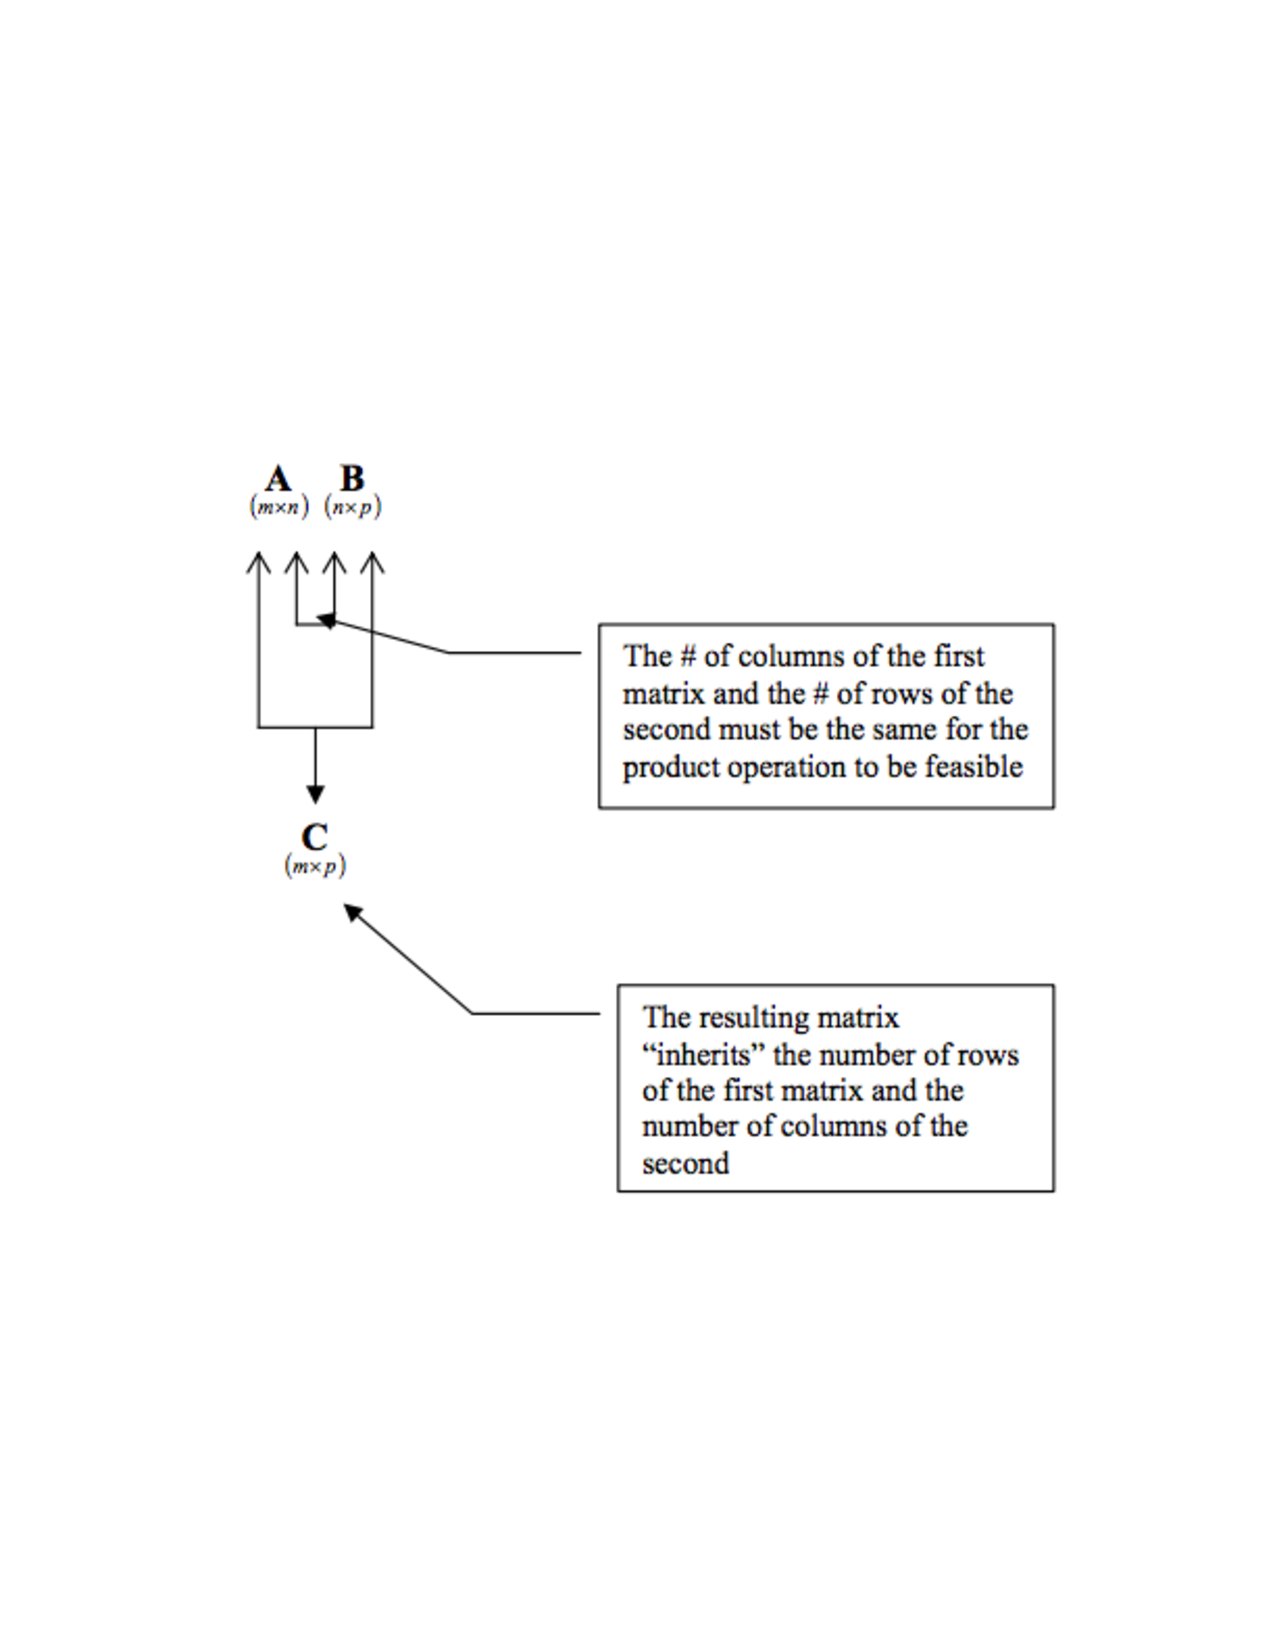
\includegraphics[scale = 0.75, trim = -150 0 0 0]{img/matrix_diagram.pdf}

The generic element of \textbf{C} is $c_{ij} = \sum_{k=1}^n a_{ik}b_{kj}$. In other words, to obtain $c_{ij}$, take the i-th row of \textbf{A} and the j-th column of \textbf{B}.
\item Example 1: 

$$
\mathbf{A} =
\begin{pmatrix}
1&-3&2&11
\end{pmatrix}
$$
$$
\textbf{B} =
\begin{pmatrix}
-3 \\
0 \\
1 \\
1
\end{pmatrix}
$$
$$
\textbf{C} = \textbf{AB} = 
(1 \times -3) + (-3 \times 0) + (2  \times 1) + (11 \times 1) = 10
$$

\item Example 2:
$$
\mathbf{A} =
\begin{pmatrix}
1&-2&4&0 \\
-1&0&5&4
\end{pmatrix}
$$
$$
\textbf{B} =
\begin{pmatrix}
1&-1&3 \\
-4&1&-1 \\
0&1&0 \\
9&6&0
\end{pmatrix}
$$
$$
\textbf{C} = \textbf{AB} = 
\begin{pmatrix}
\begin{pmatrix} 
1&-2&4&0
\end{pmatrix}\begin{pmatrix}
1 \\
-4 \\
0 \\
9
\end{pmatrix}&\begin{pmatrix} 
1&-2&4&0
\end{pmatrix}\begin{pmatrix}
-1 \\
1 \\
1 \\
6
\end{pmatrix}&\begin{pmatrix} 
1&-2&4&0
\end{pmatrix}\begin{pmatrix}
3 \\
-1 \\
0 \\
0
\end{pmatrix} \\
\begin{pmatrix} 
-1&0&5&4
\end{pmatrix}\begin{pmatrix}
1 \\
-4 \\
0 \\
9
\end{pmatrix}&
\begin{pmatrix} 
-1&0&5&4
\end{pmatrix}\begin{pmatrix}
-1 \\
1 \\
1 \\
6
\end{pmatrix}&
\begin{pmatrix} 
-1&0&5&4
\end{pmatrix}\begin{pmatrix}
3 \\
-1 \\
0 \\
0
\end{pmatrix}
\end{pmatrix}
=
\begin{pmatrix}
9&1&5 \\
35&30&-3
\end{pmatrix}
$$
\end{itemize}

\section{More Properties}
\begin{enumerate}
\item $\mathbf{IA}=\mathbf{AI}=\mathbf{A}$
\item $\mathbf{(AB)C}=\mathbf{A(BC)}$
\item $\mathbf{A(B+C)}=\mathbf{AB}+\mathbf{AC}$
\item $\mathbf{(B+C)A}=\mathbf{BA}+\mathbf{CA}$
\item $\mathbf{A}'\mathbf{A}$ and $\mathbf{A}\mathbf{A}'$ are both symmetric matrices
\item If 
$$
\mathbf{X} =
\begin{pmatrix}
x_1 \\
x_2 \\
... \\
x_n
\end{pmatrix}
$$
then (note how important the order is):
$$
\mathbf{X'X} =
\begin{pmatrix}
x_1&x_2&...&x_n
\end{pmatrix}
\begin{pmatrix}
x_1 \\
x_2 \\
... \\
x_n
\end{pmatrix}\ = \sum_{i=1}^{n} x_{i}^{2}
$$
returns a scalar (specifically, a sum of squares).
In contrast: 
$$
\mathbf{XX'} = 
\begin{pmatrix}
x_{1}^{2}&x_1x_2&...&x_1x_n \\
x_2x_1&x_{2}^{2}&...&x_2x_n \\
...&...&...&... \\
x_1x_n&x_2x_n&...&x_{n}^{2}
\end{pmatrix}
$$
is an $(n \times n)$ matrix.
\item If we have a diagonal matrix: 
$$
\textbf{A} =
\begin{pmatrix}
a_{11}&0&...&0\\
0&a_{22}&...&0\\
...&...&...&...\\
0&0&...&a_{nn}\end{pmatrix}
$$
then $\mathbf{X'AX}=\sum_{i=1}^{n}a_{ij}x_{i}^{2}$, a weighted sum of squares.
\item The identity vector, $\mathbf{i}$ is a column vector of 1s.
$$
\mathbf{i} = 
\begin{pmatrix}
1 \\
1 \\
... \\
1
\end{pmatrix}
$$
It can be used to write sums compactly, i.e., 
$$
\mathbf{X'i}=\mathbf{i'X} =
\begin{pmatrix}
x_1&x_2&...&x_n
\end{pmatrix}
\begin{pmatrix}
1 \\
1 \\
... \\
1
\end{pmatrix}
= \sum_{i=1}^{n}x_i.
$$
Note also that $\mathbf{i'i}=n$. So, the expression for the average of $x$ is $\mathbf{(i'i)^{-1}i'X}=\frac{\sum_{i=1}{n}x_i}{n}.$
\item When \textbf{a} and \textbf{b} are vectors, $\mathbf{a'b = b'a}$. This is called the \textbf{inner product} or \textbf{dot product}.

\item $\mathbf{(A')' = A}$
\item $\mathbf{(A + B)' = A' + B'}$
\item $\mathbf{(AB)' = B'A'}$
\item $\mathbf{I' = I}$
\end{enumerate}


\section{Rank of a Matrix}
\begin{itemize}
\item The column rank of a matrix \textbf{A} is the maximum number of linearly independent columns of the matrix \textbf{A}. A column is linearly independent from the other columns if we cannot write it as a linear combination of the other columns.
\begin{itemize}

\item Example: 
$$
\mathbf{a} =
\begin{pmatrix} 
1 \\ 2 \\ 2
\end{pmatrix}
,  
\mathbf{b} =
\begin{pmatrix} 
1 \\ 0 \\ 4
\end{pmatrix}
, 
\mathbf{c} =
\begin{pmatrix} 
3 \\ 4 \\ 8
\end{pmatrix}
$$
Then, \textbf{c} is not linearly independent of \textbf{a} and \textbf{b} because $\mathbf{c = 2a + b}$.
\end{itemize}

\item The row rank of a matrix \textbf{A} is the maximum number of linearly independent rows of the matrix \textbf{A}. The column rank of a matrix \textbf{A} is the maximum number of linearly independent columns of the matrix \textbf{A}. The column rank and the row rank are always equal, so we talk about the general rank of a matrix denoted as $rank(\mathbf{A})$.
\item In general, finding the rank of a matrix may not be straightforward and we often rely on computers to do the calculation.
\item For a rectangular matrix \textbf{A} with $dim(\mathbf{A}) = (R \times C)$, then $rank(\mathbf{A}) \leq min(R, C)$. 
\begin{itemize}
\item When $rank(\mathbf{A}) = min(R, C)$ exactly, we say that \textbf{A} has full rank. 
\item Otherwise, if $rank(\mathbf{A}) < min(R, C)$ we say that \textbf{A} is rank-deficient.
\end{itemize}
\item Theorems: 
\begin{enumerate}
\item $rank(\mathbf{A}) = rank(\mathbf{A'A})=rank(\mathbf{AA'})$
\item $rank(\mathbf{AB}) \leq min(rank(\mathbf{A}), rank(\mathbf{B})$
\end{enumerate}

\end{itemize}


\section{Trace of a Matrix}
\begin{itemize}
\item The trace is the sum of the elements on the main diagonal and is ONLY defined for a square matrix:
$$
tr(\mathbf{A}) = \sum_{i=1}^{n} a_{ii}
$$
\item Properties:
\begin{enumerate}
\item $tr(\mathbf{A\pm B}) = tr(\mathbf{A}) \pm tr(\mathbf{B})$
\item $tr(\mathbf{I_k}) = k$
\item $tr(\mathbf{ABC}) = tr(\mathbf{BCA}) = tr(\mathbf{CAB})$
\item $tr(\lambda) = \lambda$ if $\lambda$ is a scalar
\item $tr(\lambda \mathbf{A}) = \lambda tr(\mathbf{A})$ if $\lambda$ is a scalar
\item $tr(\mathbf{AA'}) = tr(\mathbf{A'A})$
\item $tr(\mathbf{A}) = rank(\mathbf{A})$ if \textbf{A} is idempotent
\end{enumerate}
\end{itemize}


\section{Matrix Inversion}
\begin{itemize}
\item This is the most complicated operation we do with matrices, and we will often rely on computers to do it.
\item Suppose you have a matrix \textbf{A} with generic elements $a_{ij}$. Its \textbf{inverse}, if it exists, is denoted $\mathbf{A^{-1}}$. Only square matrices can be inverted, and $dim(\mathbf{A}) = dim(\mathbf{A^{-1}})$ if $\mathbf{A^{-1}}$ exists.
\item Note that in general the generic element of $\mathbf{A^{-1}}$ will not be $a_{ij}^{-1} = \frac{1}{a_{ij}}$. However, this is true for diagonal matrices (including the identity matrix and the scalar matrix).
\item Motivation: Consider three scalars $x, y,$ and $z$. Suppose we have the following relationship:
$$
xy = z
$$
And we can solve for $x$ to get
$$
x = zy^{-1}
$$
(unless $y = 0$, in which case it is not invertible). Note also that $yy^{-1} = 1$.
\item The operation of matrix inversion has some analogies with the operation of inverting the scalar $y$ above. 
\begin{itemize}
\item In particular, the operation of matrix inversion may sometimes not be feasible. It is certainly not feasible for non-square matrices. However, it may also be infeasible for square matrices that do not satisfy an invertibility condition (detailed below).
\item Moreover, the matrix \textbf{A} and its inverse $\mathbf{A^{-1}}$ (if it exists) satisfy the identity $\mathbf{AA^{-1}=I}$. 
\end{itemize}
This suggests a first way to find the inverse of a matrix $\mathbf{A}$ (given that \textbf{A} and \textbf{I} are known). 
\item Suppose:
$$
\mathbf{A} =
\begin{pmatrix}
1&2&1 \\
-1&3&2 \\
1&0&4 
\end{pmatrix}
$$
Then its inverse (with general element $b_{ij}$) must satisfy the identity:
$$
\mathbf{AA^{-1}} =
\begin{pmatrix}
1&2&1 \\
-1&3&2 \\
1&0&4 
\end{pmatrix}
\begin{pmatrix}
b_{11}&b_{12}&b_{13} \\
b_{21}&b_{22}&b_{23} \\
b_{31}&b_{32}&b_{33} \\
\end{pmatrix}
=
\begin{pmatrix}
1&0&0 \\
0&1&0 \\
0&0&1 \\
\end{pmatrix}
$$
and $b_{ij}$ count be found by solving the system of 9 equations with 9 unknowns:
\begin{equation}
\begin{split}
b_{11} + 2b_{21} + b_{31} = 1 
\\
b_{12} + 2b_{22} + b_{32} = 0
\\
... 
\\
b_{13} + 4b_{33} = 1
\end{split}
\end{equation}


which is very time consuming.
\item Another way to find the inverse of $\mathbf{A}$ is to follow an algorithm.
\item To see how the algorithm works, we need to introduce a few more concepts. Assume we have a $(C \times C)$ matrix \textbf{A} with generic element $a_{ij}$.
\begin{enumerate}
\item The \textbf{minor} a $\mathbf{A_{ij}}$ is obtained by sweeping out the i-th row and j-th column of the matrix \textbf{A}. So if
$\mathbf{A} = 
\begin{pmatrix} 
1&2&1 \\ -1&3&2 \\ 1&0&4
\end{pmatrix} $, then $\mathbf{A_{23}} = \begin{pmatrix} 1&2 \\ 1&0 \end{pmatrix}$ and $\mathbf{A_{13}} = \begin{pmatrix} -1&3 \\ 1&0 \end{pmatrix}$.
\item The \textbf{co-factor}, which is indicated as $c_{ij} = (-1)^{i+j}|\mathbf{A}_{ij}|$. Note here that $|\textbf{A}|$ is a symbol used to define the determinant  of a matrix.
\item The \textbf{determinant} of a matrix \textbf{A} is defined as $|\textbf{A}| = \sum_{j=1}^{C} a_{ij}c_{ij} = \sum_{j=1}^{C} a_{ij}(-1)^{i+j}|\mathbf{A}_{ij}| $ for any row of column of \textbf{A}. Note that $(-1)^{i+j} = 1$ if $(i+j)$ is even and $(-1)^{i+j} = -1$ if $(i+j)$ is odd. 
\begin{itemize}
\item The determinant of a scalar is the scalar itself. 
\item If \textbf{A} is a $(2 \times 2)$ matrix, the determinant is the product of the elements in the main diagonal minus the product of the elements on the opposite diagonal.
\end{itemize}
\item Example: 
$$
\mathbf{B} = 
\begin{pmatrix}
5&1 \\
4&-3
\end{pmatrix}
$$
The minors are then $\mathbf{B_{11}} = -3$, $\mathbf{B_{12}} = 4$, $\mathbf{B_{21}} = 1$, and $\mathbf{B_{22}} = 5$. And, the determinant is:
$$
|\mathbf{B}| = (5 \times (-3)) - (1 \times 4) = -19
$$
Alternatively, we could have used the full formula above for any row or column.
\\
\\
Using the first row: 
$$ |\textbf{B}| = \sum_{j=1}^{C} b_{ij}c_{ij} = \sum_{j=1}^{C} b_{ij}(-1)^{i+j}|\mathbf{B}_{ij}| = (5(-1)^{1+1}(-3)) + (1(-1)^{1+2}4) = -19 $$
Using the second row:
$$ |\textbf{B}| = \sum_{j=1}^{C} b_{ij}c_{ij} = \sum_{j=1}^{C} b_{ij}(-1)^{i+j}|\mathbf{B}_{ij}| = (4(-1)^{2+1}1) + (-3(-1)^{2+2}5) = -19 $$
Using the first column:
$$ |\textbf{B}| = \sum_{j=1}^{C} b_{ij}c_{ij} = \sum_{j=1}^{C} b_{ij}(-1)^{i+j}|\mathbf{B}_{ij}| = (5(-1)^{1+1}(-3)) + (4(-1)^{2+1}1) = -19 $$
Using the second column:
$$ |\textbf{B}| = \sum_{j=1}^{C} b_{ij}c_{ij} = \sum_{j=1}^{C} b_{ij}(-1)^{i+j}|\mathbf{B}_{ij}| = (1(-1)^{1+2}(-3)) + (-3(-1)^{2+2}5) = -19 $$
This shows that using any row or column yields the same result. Note that the determinant is always a scalar.
\end{enumerate}
\newpage
{\Large Steps to finding the inverse:}
\begin{enumerate}
\item Calculate the minors $\mathbf{A_{ij}}$ of the matrix and the minors' determinants $|\mathbf{A_{ij}}|$.
\item Calculate the co-factors $c_{ij}$ associated to each minor using $c_{ij} = (-1)^{i+j}|\mathbf{A_{ij}}|$.
\item Create a matrix of co-factors \textbf{C} with generic elements $c_{ij}$.
\item Transpose \textbf{C}. This is so-called \textbf{adjoint} matrix of \textbf{A}, i.e. $\mathbf{C'}=adj(\mathbf{A})$
\item Calculate the determinant $|\mathbf{A}|$ using any row or column of \textbf{A}.
\item The define $\mathbf{A^{-1}}=\frac{1}{|\mathbf{A}|}adj(\mathbf{A})$
\end{enumerate}
\item Example:
$$
\mathbf{A}=
\begin{pmatrix}
1&2&1 \\
-1&3&2 \\
1&0&4 
\end{pmatrix}
$$
\textbf{Step 1:}
\\
$$
\mathbf{A_{11}}=
\begin{pmatrix}
3&2 \\
0&4 
\end{pmatrix}
,  
\mathbf{A_{12}}=
\begin{pmatrix}
-1&2 \\
1&4
\end{pmatrix}
,  
\mathbf{A_{13}}=
\begin{pmatrix}
-1&3 \\
1&0 
\end{pmatrix}
$$
$$
\mathbf{A_{21}}=
\begin{pmatrix}
2&1 \\
0&4 
\end{pmatrix}
,  
\mathbf{A_{22}}=
\begin{pmatrix}
1&1 \\
1&4
\end{pmatrix}
,  
\mathbf{A_{23}}=
\begin{pmatrix}
1&2 \\
1&0 
\end{pmatrix}
$$
$$
\mathbf{A_{31}}=
\begin{pmatrix}
2&1 \\
3&2 
\end{pmatrix}
,  
\mathbf{A_{32}}=
\begin{pmatrix}
1&1 \\
-1&2
\end{pmatrix}
,  
\mathbf{A_{33}}=
\begin{pmatrix}
1&2 \\
-1&3 
\end{pmatrix}
$$

\textbf{Step 2:}
$$
|\mathbf{A}_{11}| = 12, |\mathbf{A}_{12}| = -6, |\mathbf{A}_{13}| = -3,  
$$
$$
|\mathbf{A}_{21}| = 8, |\mathbf{A}_{22}| = 3, |\mathbf{A}_{23}| = -2,  
$$
$$
|\mathbf{A}_{31}| = 1, |\mathbf{A}_{32}| = 3, |\mathbf{A}_{33}| = 5
$$
and so:
$$
c_{11} = 12,  c_{12} = 6,  c_{13} = -3 
$$
$$
c_{21} = -8,  c_{22} = 3,  c_{23} = 2
$$
$$
c_{31} = 1,  c_{32} = -3,  c_{33} = 5
$$

\textbf{Step 3:}
$$
\mathbf{C} = 
\begin{pmatrix}
12&6&-3 \\
-8&3&2 \\
1&-3&5
\end{pmatrix}
$$

\textbf{Step 4:}
$$
adj(\mathbf{A})=\mathbf{C'}=
\begin{pmatrix}
12&-8&1 \\
6&3&-3 \\
-3&2&5
\end{pmatrix}
$$

\textbf{Step 5:}

$$
\mathbf{A} = 
\begin{pmatrix}
1&2&1 \\
-1&3&2 \\
1&0&4
\end{pmatrix}
$$

$$
|\mathbf{A}| = \sum_{j=1}^{C} a_{ij}c_{ij} = \sum_{j=1}^{C} a_{ij}(-1)^{i+j}| \mathbf{A_{ij}}|
$$

$$
|\mathbf{A}| = (1 \times 12) + (2 \times 6) + (1 \times (-3)) = 21
$$

\textbf{Step 6:}
$$
\mathbf{A^{-1}}=\frac{1}{21} 
\begin{pmatrix}
12&-8&1 \\
6&3&-3 \\
-3&2&5
\end{pmatrix}
=
\begin{pmatrix}
\frac{4}{7}&\frac{-8}{21}&\frac{1}{21} \\
\frac{2}{7}&\frac{1}{7}&\frac{-1}{7} \\
\frac{-1}{7}&\frac{2}{21}&\frac{5}{21}
\end{pmatrix}
$$

\textbf{Step 7:}
Check that $\mathbf{AA^{-1}=I}$
\newline
(Do this on your own)
\newline

\item A matrix that is not invertible is said to be \textbf{singular}. A non-invertible matrix is one with a determinant equal to zero Equivalently, it does not have full rank. 
\item Consider a matrix that is not full rank, like:
$$
\mathbf{A} = 
\begin{pmatrix}
1&3 \\
2&6
\end{pmatrix}
$$
in which the second column can be obtained by multiplying the first column by 3. Here, the determinant is $1 \times 6 - 2 \times 3 = 0$ and hence the matrix is not invertible.
\item Properties for Inverses:
\begin{enumerate}
\item $\mathbf{(A^{-1})^{-1} = A}$
\item $\mathbf{(A^{-1})' = (A')^{-1}}$
\item $\mathbf{(AB)^{-1} = B^{-1}A^{-1}}$
\end{enumerate}
\end{itemize}
\newpage
\section{Eigenvalues and Eigevectors}
\begin{itemize}
\item Consider the following problem. We want to find the values of the scalar $\lambda$ for which there exist vectors $\mathbf{x} \neq \mathbf{0}$ satisfying the equation:
$$
\mathbf{Ax} = \lambda\mathbf{x}
$$
\item The values of $\lambda$ that solve this equation are called the characteristics roots (or eigenvalues) of a matrix \textbf{A}. If \textbf{A} is a $(n \times n)$ matrix, there are $n$ eigenvalues $\lambda_1, \lambda_2, ..., \lambda_n$
$$
\mathbf{Ax} = \lambda\mathbf{Ix}
$$
$$
\mathbf{Ax} - \lambda\mathbf{Ix} = \mathbf{0}
$$
$$
(\mathbf{A} - \lambda\mathbf{I})\mathbf{x} = \mathbf{0}
$$
$$
|\mathbf{A} - \lambda\mathbf{I}| = \mathbf{0}
$$

Why? Assume that instead $\mathbf{B} = (\mathbf{A} - \lambda\mathbf{I})$ is invertible. Then we can write $\mathbf{Bx = 0}$, $\mathbf{B^{-1}Bx=0}$ and $\mathbf{x = 0}$, which is a contradiction (we assumed that $\mathbf{x} \neq \mathbf{0}$). 
\item The vectors associated to the eigenvalues, $\lambda_i$'s, are called eigenvectors (typically, denoted $\mathbf{v_1, v_2, ..., v_n}$).
\item Consider the following example:
$$
\mathbf{A} = 
\begin{pmatrix}
2&2 \\
2&-1
\end{pmatrix}
$$
Let's find $|\mathbf{A}-\lambda \mathbf{I}|$. We have:
$$
|\begin{pmatrix}
2-\lambda & 2 \\
2 & -1 - \lambda
\end{pmatrix}|
= -(2 - \lambda )(1+\lambda) - 4 = 0
$$
$$
\lambda^2 - \lambda - 6 = 0
$$
$$
\lambda_1 = 3, \lambda_2 = -2
$$
Now, let's find the eigenvectors. For $\lambda = 3$ we have:

$$
\begin{pmatrix}
-x_1 + 2x_2 \\
2x_1 - 4x_2
\end{pmatrix}
=
\begin{pmatrix}
0 \\
0
\end{pmatrix}
$$
i.e., $x_1 = 2x_2$. For $\lambda = -2$ we have $x_1 = \frac{-1}{2}x_2$. We need to impose a normalization constraint (otherwise we cannot pin down $x_1$ and $x_2$ separately). The typical normalization constraint is: $\mathbf{x'x}=1$, and hence we get solutions.
\newline
\newline
When $\lambda = 3$: $x_1^2 + x_2^2 = 1$, or $x_1 = \frac{2}{\sqrt[]{5}}$, $x_2 = \frac{1}{\sqrt[]{5}}$ 
\newline
\newline
When $\lambda = -2$: $x_1^2 + x_2^2 = 1$, or $x_1 = \frac{-1}{\sqrt[]{5}}$, $x_2 = \frac{2}{\sqrt[]{5}}$ 
\newline
\newline
Hence:
$$
\mathbf{v_1} =
\begin{pmatrix}
\frac{2}{\sqrt[]{5}} \\
\frac{1}{\sqrt[]{5}}
\end{pmatrix}
,  
\mathbf{v_2} =
\begin{pmatrix}
\frac{-1}{\sqrt[]{5}} \\
\frac{2}{\sqrt[]{5}}
\end{pmatrix}
$$

For a symmetric matrix, characteristic vectors corresponding to distinct characteristics roots are pairwise orthogonal. That is $\mathbf{v_iv_i'} = 1$ and $\mathbf{v_iv_j'} = 0$. This is easy to verify in our example above. Try doing it on your own.

The $(n \times n)$ matrix of eigenvectors is:
$$
\mathbf{Q} = 
\begin{pmatrix}
\mathbf{v_1}&\mathbf{v_2}&...&\mathbf{v_n}
\end{pmatrix}
$$

Now, notice that 
$$
\mathbf{Q'} = 
\begin{pmatrix}
\mathbf{v_1} \\
\mathbf{v_2} \\
... \\
\mathbf{v_n}
\end{pmatrix}
$$
And, therefore 
$$
\mathbf{QQ'} = 
\begin{pmatrix}
\mathbf{v_1'v_1}&\mathbf{v_1'v_2}&...&\mathbf{v_1'v_n} \\
 &\mathbf{v_2'v_2}&...&\mathbf{v_2'v_n} \\
 & & ... & \mathbf{v_3'v_n} \\
 & & & \mathbf{v_n'v_n}
\end{pmatrix}
$$

And so also $\mathbf{Q' = Q^{-1}}$. Therefore $\mathbf{Q}$ is said to be an orthogonal matrix.

Now write $\mathbf{AQ}$:
$$
\mathbf{AQ} =
\begin{pmatrix}
\mathbf{Av_1}&\mathbf{Av_2}&...&\mathbf{Av_n}
\end{pmatrix}
=
\begin{pmatrix}
\lambda\mathbf{v_1}&\lambda\mathbf{v_2}&...&\lambda\mathbf{v_n}
\end{pmatrix}
= \mathbf{Q\Lambda}
$$
Where $\mathbf{\Lambda}$ is a diagonal matrix with the eigenvalues on the main diagonal. We conclude that:
$$
\mathbf{Q'AQ = Q'Q\Lambda = \Lambda}
$$
The operation is called the diagonalization of a matrix \textbf{A}. We have found a matrix \textbf{Q} such that the transformation $\mathbf{Q'AQ}$ produces a diagonal matrix with \textbf{A}'s characteristic roots along the main diagonal.
\item Useful things to know:
\begin{enumerate}
\item For a square matrix \textbf{A}, the product of the eigenvalues is equal to the determinant of the matrix.
\item For a square matrix \textbf{A}, the rank of \textbf{A} is equal to the number of nonzero eigenvalues. 
\end{enumerate}
\item Consider now an idempotent matrix \textbf{M}. For example:
$$
\mathbf{M} =
\begin{pmatrix}
\frac{1}{2}&\frac{-1}{2} \\ 
\frac{11}{2}&\frac{1}{2} 
\end{pmatrix}
$$
It's easy to show that the only eigenvalues that solve the characteristics equation $\mathbf{Mx} = \lambda\mathbf{x}$ are $\lambda_1 = 0$ and $\lambda_2 = 1$. In general, one can show that an idempotent $(n \times n)$ matrix of rank $k \leq n$ has $k$ eigenvalues equal to 1 and $(n-k)$ eigenvalues equal to 0. 
What about eigenvectors of \textbf{M}? 
\newline
Let's find them for our example:
$$
\mathbf{v_1} =
\begin{pmatrix}
\frac{1}{\sqrt[]{2}} \\
\frac{1}{\sqrt[]{2}}
\end{pmatrix}
,  
\mathbf{v_2} =
\begin{pmatrix}
\frac{1}{\sqrt[]{2}} \\
\frac{-1}{\sqrt[]{2}}
\end{pmatrix}
$$
Now write \textbf{MQ}:
$$
\mathbf{MQ} =
\begin{pmatrix}
\mathbf{Mv_1}&\mathbf{Mv_2}&...&\mathbf{Mv_n}
\end{pmatrix}
=
\begin{pmatrix}
\lambda_1\mathbf{v_1}&\lambda_2\mathbf{v_2}&...&\lambda_n\mathbf{v_n}
\end{pmatrix}
= \mathbf{Q\Lambda}
$$
Where in our case $\mathbf{\Lambda}$ is a diagonal matrix that has $k$ 1's and $(n-k)$ 0's in the main diagonal. And also 
$$
\mathbf{Q'MQ} = \mathbf{\Lambda}
$$
is the diagonalization of \textbf{M}.
\end{itemize}



\section{Matrix Calculus}
\begin{itemize}
\item Suppose you have the following:
$$
\begin{pmatrix}
\beta_1 \\
\beta_2 \\
... \\
\beta_k
\end{pmatrix}
,
\begin{pmatrix}
c_1 \\
c_2 \\
... \\
c_k
\end{pmatrix}
,
\begin{pmatrix}
a_{11}&a_{12}&...&a_{1k} \\
a_{21}&a_{22}&...&a_{2k} \\
...&...&...&... \\
a_{k1}&a_{k2}&...&a_{kk} \\
\end{pmatrix}
$$

\item And then you have the mapping $ y = f(\beta) $. The objective is to find the derivative of $y$ with respect to $\beta$. This can be defined as the vector:

$$
\frac{\partial y}{\partial \beta} = \frac{\partial f(\beta)}{\partial \beta} = 
\begin{pmatrix}
\frac{\partial f(\beta)}{\partial \beta_1} \\
\frac{\partial f(\beta)}{\partial \beta_2} \\
... \\
\frac{\partial f(\beta)}{\partial \beta_k}
\end{pmatrix}
$$

This is the so-called vector of gradients.

\item We will consider the following mappings:
$$
y = f(\beta) = \mathbf{c'\beta = \beta'c} = \sum_{i=1}^{k} \beta_i c_i
$$
$$
y = f(\beta) = \mathbf{\beta'A\beta}
$$
\item The corresponding gradient vectors are:
$$
\frac{\partial y}{\partial \beta} = \frac{\partial \beta'\mathbf{c}}{\partial \beta} = \frac{\partial \mathbf{c'\beta}}{\partial \beta} = 
\begin{pmatrix}
\frac{\partial (\beta_1 c_1 + \beta_2 c_2 + .. + \beta_k c_k)}{\partial \beta_1} \\
\frac{\partial (\beta_1 c_1 + \beta_2 c_2 + .. + \beta_k c_k)}{\partial \beta_2} \\
... \\ 
\frac{\partial (\beta_1 c_1 + \beta_2 c_2 + .. + \beta_k c_k)}{\partial \beta_k} 
\end{pmatrix}
=
\begin{pmatrix}
c_1 \\
c_2 \\
... \\
c_k
\end{pmatrix}
= \mathbf{c}
$$

$$
\frac{\partial y}{\partial \beta} = \frac{\partial \beta'\mathbf{A}\beta}{\partial \beta} = \mathbf{A\beta + A'\beta} = 2\mathbf{A\beta}
$$
This last equation is true only if \textbf{A} is a symmetric matrix.


\end{itemize}

\section{The OLS Problem}
\begin{itemize}
\item Consider a model with $k$ regressors for $N$ individuals $(N > k)$. Write the regression model for each individual:
\begin{equation*}
\begin{split}
y_1 = \beta_0 + \beta_1 x_{11} + \beta_2 x_{12} + ... + \beta_k x_{1k} \\
y_2 = \beta_0 + \beta_1 x_{21} + \beta_2 x_{22} + ... + \beta_k x_{2k} \\
\vdots \quad  \quad \quad \quad \vdots \quad \quad \quad \quad \vdots \\
y_n = \beta_0 + \beta_1 x_{n1} + \beta_2 x_{n2} + ... + \beta_k x_{nk} \\
\end{split}
\end{equation*}
\item Note than in $x_{ij}$, the $i$ subscript index the individual or unit, and the $j$ subscript the variable. This can be put in matrix format as:
$$
\begin{pmatrix}
y_1 \\
y_2 \\
... \\
y_n
\end{pmatrix}
=
\begin{pmatrix}
1&x_{11}&x_{12}&...&x_{1k} \\
1&x_{21}&x_{22}&...&x_{2k} \\
...&...&...&...&... \\
1&x_{n1}&x_{n2}&...&x_{nk} \\
\end{pmatrix}
\begin{pmatrix}
\beta_1 \\
\beta_2 \\
... \\
\beta_k
\end{pmatrix}
+
\begin{pmatrix}
u_1 \\
u_2 \\
... \\
u_n
\end{pmatrix}
$$

Or more compactly as:
$$
\mathbf{y = X \beta + u}
$$
\item The OLS problem is to solve:
$$
\min\limits_\beta f(\hat{\beta)} =  \sum_{i=1}^{n} \mathbf{\hat{u}_{i}^{2}} = \mathbf{\hat{u}'\hat{u}} = \mathbf{(y - X\hat{\beta})'(y - X\hat{\beta})} = \mathbf{(y' - \hat{\beta}'X')(y-X\hat{\beta})} = \mathbf{y'y - y'X\hat{\beta} - \hat{\beta}X'y + \hat{\beta}'X'X\hat{\beta}}
$$
\item To find the minimum, take the derivative of this objective and set equal to zero (i.e. $\frac{\partial f(\hat{\beta}}{\partial \hat{\beta}} = 0$):
$$
0 = \frac{\partial(\mathbf{y'y - y'X\hat{\beta} - \hat{\beta}X'y + \hat{\beta}'X'X\hat{\beta}})}{\partial \hat{\beta}}
$$
$$
0 = \frac{\partial(\mathbf{y'X\hat{\beta}})}{\partial \hat{\beta}} - \frac{\partial (\mathbf{\hat{\beta}X'y})}{\partial \hat{\beta}} + \frac{\partial (\mathbf{\hat{\beta}'X'X}\hat{\beta})}{\partial \hat{\beta}}
$$
$$
0 = \mathbf{-X'y - X'y + 2X'X\hat{\beta}} = \mathbf{-2X'y + 2X'X\hat{\beta}} = \mathbf{-X'y + X'X\hat{\beta}}
$$
Or:
$$
\mathbf{X'X\hat{\beta} = X'y}
$$
\item If $\mathbf{X'X}$ is invertible,then we can pre-multiply both sides by $\mathbf{(X'X)^{-1}}$ to yield the OLS solution:
$$
\mathbf{\hat{\beta} = (X'X)^{-1}X'y}
$$
\item When $\mathbf{X'X}$ is not invertible, does it prevent solving the OLS problem? Only when it does not have full rank. Recall the theorem:
$$
rank(\mathbf{A}) = rank(\mathbf{A'A}) = rank(\mathbf{AA'})
$$
\item This means that the rank of $\mathbf{X'X}$  is equal to the rank of the matrix of the covariates $\mathbf{X}$. Thus, if we have columns of \textbf{X} that are not linearly independent, the matrix $\mathbf{X'X}$  cannot be inverted. This is what we call multicollinearity. 
\end{itemize}

\end{document}
\bibliography{mathcamp}
